% Template for ISBI-2016 paper; to be used with:
%          spconf.sty  - ICASSP/ICIP LaTeX style file, and
%          IEEEbib.bst - IEEE bibliography style file.
% --------------------------------------------------------------------------
\documentclass{article}
\usepackage{spconf,amsmath,graphicx}
\usepackage{amsfonts}
\usepackage[utf8]{inputenc}
\usepackage[francais]{babel}
\usepackage{hyperref}

% Example definitions.
% --------------------
\def\x{{\mathbf x}}
\def\L{{\cal L}}

% Title.
% ------
\title{Nuclei Segmentation in Histopathology
  images using Deep Neural Networks}
%
% Single address.
% ---------------
%%% Not too sure about who to thank, I guess me, you, phil, and ema?
%\name{Peter Naylor, Marick Lae, Fabien Reyal and Thomas Walter\thanks{}}
%\address{(1)   MINES ParisTech, PSL Research University, CBIO - Centre de bio-informatique, 35 rue St Honoré 77300 Fontainebleau, France
%(2)   Institut Curie, 75248 Paris Cedex, France
%(3)   INSERM U900, 75248 Paris Cedex, France}
%
% For example:
% ------------
%\address{School\\
%	Department\\
%	Address}
%
% Two addresses (uncomment and modify for two-address case).
% ----------------------------------------------------------
%\twoauthors
%  {A. Author-one, B. Author-two\sthanks{Thanks to XYZ agency for funding.}}
%	{School A-B\\
%	Department A-B\\
%	Address A-B}
%  {C. Author-three, D. Author-four\sthanks{The fourth author performed the work
%	while at ...}}
%	{School C-D\\
%	Department C-D\\
%	Address C-D}
%
% More than two addresses
% -----------------------

\name{Peter Naylor$^{1,2,3}$\sthanks{Peter Naylor has received a PhD
  fellowship from the Ligue contre le Cancer. } \qquad Marick La\'e$^{4}$
  \qquad Fabien Reyal$^{2}$\qquad Thomas Walter$^{1,2,3}$}

\address{$^{1}$MINES ParisTech, PSL Research University, CBIO - Centre
  de Bioinformatique,\\ 
  35 rue St Honoré 77300 Fontainebleau, France \\
$^{2}$Institut Curie, 75248 Paris Cedex, France\\
$^{3}$INSERM U900, 75248 Paris Cedex, France\\
$^{4}$Service de Pathologie, Institut Curie, 75248 Paris Cedex, France}
%
\begin{document}
%\ninept
%
\maketitle
%
\begin{abstract}
%The abstract should appear at the top of the left-hand column of text, about
%0.5 inch (12 mm) below the title area and no more than 3.125 inches (80 mm) in
%length.  Leave a 0.5 inch (12 mm) space between the end of the abstract and the
%beginning of the main text.  The abstract should contain about 100 to 150
%words, and should be identical to the abstract text submitted electronically
%along with the paper cover sheet.  All manuscripts must be in English, printed
%in black ink.
\end{abstract}
%
\begin{keywords}
Deep Learnnig, Convolutional Neural Networks, Nuclei Segmentation,
Histpathology, Digital Pathology, Breast Cancer, Cellular Phenotyping
\end{keywords}
%
\section{Introduction}
\label{sec:intro}

% images in cancer research, histopathology --> digital pathology
Today, large sequencing approaches build the main body of cancer
research programs and they have revolutionized our understanding of
the molecular basis of cancer. In clinical practice however,
molecular profiling is paralleled with the more traditional
(and mostly manual) analysis of stained histological tumor
sections. With the avent of digital pathology, i.e. the scanning and
digital storage of diseased tissue sections, it is now possible to
build tools for the quantitative and automatic analysis of these
complex and informative image data. Indeed, this is a very promising
approach for several reasons: image based approaches
provide us with spatial information that is absent in genomic,
transcriptomic and epigenetic studies of cancer. In addition they
allow analysis of individual cells, such that it is possible to study
cellular heterogeneity. Cellular heterogeneity has been acknowledged
to be of major importance in cancer research and treatment. Also, it
is possible to analyze cells in terms of morphology and phenotype,
which brings in a complementary piece of functionally relevant
information.  

% two approaches: CAD vs. understanding
For these reasons, analysis of histopathology data has received much
attention over the last years. Most of these works are in the frame of
Computer Aided Diagnosis (CAD) and aim at automatically performing the
task of a human pathologist or at assisting in the diagnosis. For such
a task, the nature of the features according to which a certain
classification or detection task is solved is mostly
irrelevant. A conceptually different approach is to derive biologically
relevant features, such as phenotype distributions, spatial cell type
distributions or heterogeneity measures from the tissue data in order to reach some
understanding as of which biological features can be predictive for
clinical variables such as resistance to treatment or relapse
probability. 

% segmentation is the bottleneck of cellular phenotyping in cancer
% tissues. 
In this latter case, one of the essential steps is to
segment nuclei from tissue images in order to be able to
assign them a cell type or phenotypic label and to evaluate their
spatial distribution. We concentrate on nuclei, as they are indicative
of many cellular phenotypes\cite{Chow2012}, and their morphology is 
currently used by pathologists in order to
identify the mitotic index and the level of nuclear
pleomorphism\cite{Elston1991}. 

Yet, segmentation of nuclei is a
complicated task: tissue type, staining differences and cell type
convey them different visual characteristics, which makes it very difficult to
design traditional image segmentation algorithms that work
satisfactorily for all of these different cases. On the other hand,
deep learning algorithms have been used recently with great success to
complex segmentation tasks in biology\cite{Ciresan2012,UNet}. 

The contribution of this paper is three-fold: (1) we have generated a
ground truth of annotated images containing segmentation results for
more than 2000 cells. The dataset can be used by the scientific
community. (2) We apply a deep neural network end-to-end strategy and
demonstrate the superiority of this approach with respect to
previously proposed simpler architectures. (3) We propose a
post-processing strategy of the posterior probabilities provided by
the network. This post-processing strategy is based on mathematical
morphology and has a rigorous interpretation as to when objects are to
be split. 

\section{Related work}
\label{sec:related}
Image segmentation and object recognition in medical imagining have 
been tackled for many years and many approaches have been found. 
Methods based on mathematical morphological operators have been 
widely used and applied for segmentation and feature extraction, 
however such methods rely on the user to manually define the 
information that is relevant for his task \cite{irshad2014methods}. 
Segmentation methods based on a strong priori information are also 
possible and yield comparable results in terms of accuracy, in 
\cite{ranefall2016fast} they segment the picture using a ellispe fit 
which is considerably faster than other state of the art methods. Graph-
based tools for segmentation are also possible in histopathology 
\cite{ta2009graph}. \cite{manivannanlocal} focus on gland 
segmentation, they achieve good results by predicting image patches as 
a whole, via a classification scheme. The output confidence vector is 
then preprocessed to obtain the final segmentation. Alternative methods 
have arisen from the achieving Convolutional neural networks 
\cite{lecun}, in particular strong incentive rose with the very impressive 
results that they achieved in the pascal voc challenge with 
\cite{ImageNet}. Recent advances in deep neural network, and in 
particular in their optimization have made them become the state-of-the-
art model for object recognition.  Deep neural network have also been 
used for different task and have yielded very impressiv results, we can think of 
semantic segmentation problems, where \cite{long2015fcn} use "de-
convolution layers" and up-sampling in order to identify and precisely 
locate objects within a picture. Different architecture arising from 
different intuition are also possible and have been applied in this paper.



Talk about related work.

\section{DataSet}
\label{sec:dataset}

%% Contribution as a dataset, small introduction
One of the main contributions of this paper is the now public available 
nuclei detection dataset within HE stainned histopathology images which 
can be found at website %\url{www.cbio.ensmp.fr:/pnaylor/download/dataset.zip} 
(not a true address). This annotated dataset provides images clustered by 
patients. Each patient has at least 3 annotated $512 \times 512$ HE 
stainned histopathology images with their associated ground truth. Each 
ground truth image is a $512 \times 512$ image where each pixel value above 
$0$ is considered as a pixel belonging to a nuclei. The differences in 
values of these pixels denote different nucleus, such an annotation can 
be used in several processing step which does or doesn't take into 
account clutered nuclei. See figure \ref{fig:annotation} for an example of 
three annotated images. This annotation was conducted via the help of 
the software ITK-snap, \cite{py06nimg} http://www.itksnap.org, and were annotated by the authors of the paper.


%% Data set creation procedure
These patients were randomly picked from an unpublished study on
tripple negative breast cancer. For each of these patients we had access
to their biopsy sample as a whole slide image (WSI). WSI enables a
medical practitionner to digitize the huge amount of information that
can be found in glass slides. WSI can be up to 60 GB big
uncompressed and can't be stored in RAM on a standard computer. Given
the WSI of a patient, we randomly cropped $512 \times 512$ samples 
from the WSI. %% explain that we choose the tissue area? 
3 to 7 images were choosen from the randomly sampled images to try and give the most diversed dataset among these patients. Once the samples were choosen, we fully annotated each nuclei via the software ITK-snap and touching nuclei are differentiate via a different annotation value.

%%Data set description 
In this data set we have annotated a considerous amount of cells, 
including normal breast cells (epithelial and lobule cells),  cancerous 
breast cells, fibroblasts,  endothelial cells, fat cells, macrophage cells and 
inflammatory cells (lymphocytes and plasmocytes). For the moment, cell types have not been seperated, which means that in this dataset every annotation corresponds to a global type: cell. 

\begin{itemize}
\item Number of images: 33 \\
\item Number  of cells: 2754 \\
\item Maximum number of cells in one sample: 293 \\
\item Minimum number of cells in one sample: 5 \\
\item Mean number of cells: 83 \\
\item Standard deviation of number of cells: 63 \\
\end{itemize}

\section{Methodology}
\label{sec:method}
%% Segmentation task
Let A be the space of RGB images, A can typically be 
$\mathbb{R}^{n \times p \times 3}$ and let B the space B the space of annotation 
images, in our case $\{0,1\}^{n \times p}$. We have a set of 
$(A_l,B_l)_{l \in [1, N]}$ for a supervised learning approach. Our goal is 
a prediction task 
named as semantic segmentation, we wish to maximize the prediction of 
an unseen element belonging to B given an new element in A. We maximize 
thus prediction by modelizing our prediction function as the softmax output of a deep neural 
network. We find the model parameters by minimizing a log loss function 
defined as:
 $\frac{1}{\sum_{i,j}w_{ij}} \sum_{i,j} \sum_k w_{i,j} t_{i,j,k} \log (\widehat{p_{i,j,k}})$
, where $k$ designates a certain label, $w_{i,j}$ is a 
certain weight given to pixel $i,j$, $t_{i,j,k}$ is equal to 1 if pixel $i,j$ is 
of class $k$ and $\widehat{p_{i,j,k}}$ designates the estimated probability 
of pixel $i,j$ of being $k$ via the softmax output of the neural network.
We minimize the loss function via stochastic gradient descent.

%% Validation scheme
We have our training set $(A_l,B_l)_{l \in [1, N]}$ where N is equal to 
33, how ever each element $A_l$ belongs to a certain patients and 
several elements $A_l$ can belong to the same patient. As we are 
dealing with histopathology images, it is know that samples can widely 
vary from one patient to the other. We thus validate our model by a 
leave one patient out scheme. Our validation scheme is as followed, for a 
given set of hype parameters, we 
train our model on every patient except one that is used for validation. 
Our final score is averaged over all patients.
Several metrics assess the quality of the model, the accuracy, the 
F1 score and a performance score which is the mean between the 
true positive rate and the true negative rate.

%% Data augmentation and Hyper parameter training: Training scheme
%% Check number of images and number of transformations
To train our models, as the number of available annotated is scarse, we 
used a great number of transformation for the data augmentation. From 
a original size of 33 annotated images, adding flips, rotations, bluriness 
and random elastic deformations enabled us to have more then 
$400 000$ training images. 
We also try out several hyperparameter configurations: the learning rate and 
momentum for the stochastic gradient descent, the weight decay value.  
In practice, we found that hyperparameters tuning didn't influence the 
scores much, the exepction being the learning rate. If the learning rate 
was not of the right magnitude the given network did not seem to learn. 
We therefore fixed the momentum to be 0.9 and the weight decay to be 
$5.10^{-5}$ for all of the experiences, the learning rate was tunned 
according to the model choosen.
We also experienced with different 
initialization value and if possible, we also considered pretrained layers. 
Using pretrained layers made learning more efficient and made score 
values more robust.

%% Mathematical Morphology
The results obtained by the Deep Neural Network were encouraging, but
touching nuclei were often segmented as one single object. This is not
surprising, as the error at a pixel level seems very minor, and no
shape prior is used in the model. Solving this issue by weighting the
error term for pixels between objects did not solve the issue for our
case (data not shown). However, we did observe that for touching and
even partially overlapping nuclei, the posterior probability at the
nucleus border is systematically lower than in
the putative center of the nucleus, but may still be larger than
typically applied thresholds.This leads to the following rationale. As in the center of nuclei, the
posterior probability is maximal, we can readily assume that the local
maxima of the posterior correspond to putative nuclei, which we call candidates. Let
$\mathcal{X}=(x_1,x_2,\ldots,x_N)$ be a path that joins two candidates
(i.e. $\forall i, \ x_i$ and $x_{i+1}$ are neighbor pixels) and
$\mathcal{P}=(p_1,p_2,\ldots,p_N)$ the corresponding posterior
probabilities. Without loss of generality, we assume $p_1\leq P_N$.
We define for each path $\mathcal{X}$ a cost
$C(\mathcal{P})=\max_{i=2 \ldots N}{p_1-p_i}$, which is the maximal
decrease in posterior probability along the path, when starting from
the candidate with lower probability.  Considering all paths joining two
candidates, we can now state a criterion that allows us to decide whether to
perform a split (and thus accept the candidates as being different
nuclei) or not: if all the paths involve a decrease in probability
larger than a parameter $\lambda$, we will perform a
split. Conversely, if we can find a path that joins the two candidates
with a probability decrease smaller or equal to $\lambda$, no split
will be performed: we argue that in this case, it is probably one
single object. Hence, the split is performed if: 
\begin{equation}
\min_{\mathcal{P}}C(\mathcal{P}) = \min_{\mathcal{P}} \{\max_{i=2
  \ldots N}{p_1-p_i}\} > \lambda
\end{equation}
where $\lambda$ is a free parameter. This is actually nothing else
than the morphological dynamics\cite{Grimaud1992}. The actual split
locations are thus obtained by applying the watershed algorithm,
starting from the local maxima of the posterior probability map with
morphological dynamics larger than a free parameter $\lambda$. 

To speed up this procedure, we have developed an algorithm that
performs selection and Watershed algorithm in a single pass by
selectively building the Watershed line or fusing the regions,
depending on the morphological dynamic at the moment at which two
regions get in contact. This algorithm will be made publicly available
through the open-source software scikit-image\cite{scikit-image}, in which we implemented
all the steps which were not related to deep learning. 



\section{Different architectures/Results}
\label{sec:results}
We experience with 3 known arhitectures in semantic segmentation, named PangNet, Fully Convolutionnal Net (FCN) and DeconvNet. The most basic architecture, PangNet, consists of 4 
convolutionnal layer where each convolutionnal layer has 8 feature map, for more information please refer to \cite{pang2010cell}. 
This net, being not deep, has the advantage of being less 
computationnally intensive. FCN is a first attempt of applying "deep 
feature" representations to the task of semantic segmentation. This 
archicture has the advantage of re-using a classical deep learning 
architecture with added on upsampling layer and skip layers. The 
upsampling layers enable the network to learn a pixel level classification 
and the skip layers enable the network to fuse different levels of 
abstraction to the final prediction. This model can be fine tuned with a 
set of pretrained-weights extracted from the classical deep learning 
architecture, for a more detailed explaination please refer to \cite{long2015fcn}. DeconvNet is also based on a classical architecture, 
however, in this network their are no skip layer as one intends to learn 
the proper upsampling threw repeated deconvolution and convolution 
layers. This model can also be fine tuned, for more information please 
refer to the original paper \cite{noh2015learning}. We did not
ensemble classifier as suggested in 
\cite{noh2015learning} as our FCN and DeconvNet classifier achieve very similar scores on the test sets.
% The final architecture that we tried is the UNet. This network combines 
%both contribution of the above networks, the UNet has a similar 
%architecture to the DeconvNet with skip layers.
\section{Result and discussion}
\label{sec:result}
We conducted our experiments on GPUs via the caffe framework, \cite{jia2014caffe}. We present our results in table \ref{tab:res} where we averaged the metrics other all left out patients. We also added, for illustration purposes \ref{fig:prediction}, image prediction and associated probability maps to evaluate some differences between the classifiers. We notice that the simpler net, PangNet seems to have learnt simple rules such as color information. As we can not notice by the "holes" in the probability map when the interior of the cell is brighter. On the contrary, deeper nets as FCN and DeconvNet have learnt deeper features and seem capable of recognizing whole cells. .
\begin{table}
\begin{tabular}{|c|c|c|c|}
\hline
  & PangNet & DeconvNet & FCN \\
 \hline
Accuracy  &       0.936 & 0.968 &0.958  \\
IU   &    0.759 &     0.856 & 0.857 \\
Recall     &       0.744  &     0.856 & 0.855 \\
Precision   &       0.741 &     0.858 & 0.878\\
F1    &       0.742 &     0.856 & 0.866 \\
TP       &       0.744 &     0.856 & 0.855  \\
TN      &       0.963 &     0.981 &  0.977\\
Performance    &       0.853 &     0.918 & 0.916\\
Pixel error  &  0.063 &     0.032 & 0.042\\
\hline
\end{tabular}
\caption{Results}
\label{tab:res}
\end{table}

%%with Unet
%\begin{tabular}{|c|c|c|c|c|c|}
% & UNet & PangNet & DeconvNet & FCN & Ensemble \\
%\hrule
%Accuracy &       0.89 &       0.936 & 0.968 &0.958 & \\
%IU   &       0.70 &       0.759 &     0.856 & 0.857 &\\
%Recall    &       0.75 &       0.744  &     0.856 & 0.855 &\\
%Precision    &       0.64 &       0.741 &     0.858 & 0.878&\\
%F1       &       0.69 &       0.742 &     0.856 & 0.866&  \\
%TP             &       0.75 &       0.744 &     0.856 & 0.855 & \\
%TN             &       0.92 &       0.963 &     0.981 &  0.977&\\
%Performance    &       0.84 &       0.853 &     0.918 & 0.916&\\
%Pixel error  &       0.11 &       0.063 &     0.032 & 0.042&\\
%\end{tabular}


%\section{Formatting your paper}
%\label{sec:format}
%
%All printed material, including text, illustrations, and charts, must be kept
%within a print area of 7 inches (178 mm) wide by 9 inches (229 mm) high. Do
%not write or print anything outside the print area. The top margin must be 1
%inch (25 mm), except for the title page, and the left margin must be 0.75 inch
%(19 mm).  All {\it text} must be in a two-column format. Columns are to be 3.39
%inches (86 mm) wide, with a 0.24 inch (6 mm) space between them. Text must be
%fully justified.
%
%\section{PAGE TITLE SECTION}
%\label{sec:pagestyle}
%
%The paper title (on the first page) should begin 1.38 inches (35 mm) from the
%top edge of the page, centered, completely capitalized, and in Times 14-point,
%boldface type.  The authors' name(s) and affiliation(s) appear below the title
%in capital and lower case letters.  Papers with multiple authors and
%affiliations may require two or more lines for this information.
%
%\section{TYPE-STYLE AND FONTS}
%\label{sec:typestyle}
%
%To achieve the best rendering both in the proceedings and from the CD-ROM, we
%strongly encourage you to use Times-Roman font.  In addition, this will give
%the proceedings a more uniform look.  Use a font that is no smaller than nine
%point type throughout the paper, including figure captions.
%
%In nine point type font, capital letters are 2 mm high.  If you use the
%smallest point size, there should be no more than 3.2 lines/cm (8 lines/inch)
%vertically.  This is a minimum spacing; 2.75 lines/cm (7 lines/inch) will make
%the paper much more readable.  Larger type sizes require correspondingly larger
%vertical spacing.  Please do not double-space your paper.  True-Type 1 fonts
%are preferred.
%
%The first paragraph in each section should not be indented, but all the
%following paragraphs within the section should be indented as these paragraphs
%demonstrate.
%
%\section{MAJOR HEADINGS}
%\label{sec:majhead}
%
%Major headings, for example, "1. Introduction", should appear in all capital
%letters, bold face if possible, centered in the column, with one blank line
%before, and one blank line after. Use a period (".") after the heading number,
%not a colon.
%
%\subsection{Subheadings}
%\label{ssec:subhead}
%
%Subheadings should appear in lower case (initial word capitalized) in
%boldface.  They should start at the left margin on a separate line.
% 
%\subsubsection{Sub-subheadings}
%\label{sssec:subsubhead}
%
%Sub-subheadings, as in this paragraph, are discouraged. However, if you
%must use them, they should appear in lower case (initial word
%capitalized) and start at the left margin on a separate line, with paragraph
%text beginning on the following line.  They should be in italics.
%
%\section{PRINTING YOUR PAPER}
%\label{sec:print}
%
%Print your properly formatted text on high-quality, 8.5 x 11-inch white printer
%paper. A4 paper is also acceptable, but please leave the extra 0.5 inch (12 mm)
%empty at the BOTTOM of the page and follow the top and left margins as
%specified.  If the last page of your paper is only partially filled, arrange
%the columns so that they are evenly balanced if possible, rather than having
%one long column.
%
%In \LaTeX, to start a new column (but not a new page) and help balance the
%last-page column lengths, you can use the command ``$\backslash$pagebreak'' as
%demonstrated on this page (see the \LaTeX\ source below).
%
%\section{PAGE NUMBERING}
%\label{sec:page}
%
%Please do {\bf not} paginate your paper.  Page numbers, session numbers, and
%conference identification will be inserted when the paper is included in the
%proceedings.
%
%\section{ILLUSTRATIONS, GRAPHS, AND PHOTOGRAPHS}
%\label{sec:illust}
%
%Illustrations must appear within the designated margins.  They may span the two
%columns.  If possible, position illustrations at the top of columns, rather
%than in the middle or at the bottom.  Caption and number every illustration.
%All halftone illustrations must be clear black and white prints.  If you use
%color, make sure that the color figures are clear when printed on a black-only
%printer.
%
%Since there are many ways, often incompatible, of including images (e.g., with
%experimental results) in a \LaTeX\ document, below is an example of how to do
%this \cite{Lamp86}.

% Below is an example of how to insert images. Delete the ``\vspace'' line,
% uncomment the preceding line ``\centerline...'' and replace ``imageX.ps''
% with a suitable PostScript file name.
% -------------------------------------------------------------------------
\begin{figure}[htb]
\begin{minipage}[b]{.48\linewidth}
  \centering
  \centerline{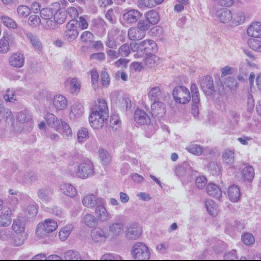
\includegraphics[width=4.0cm]{RGB_1}}
%  \vspace{1.5cm}
  \centerline{Sample from patient 498959}\medskip
\end{minipage}
\hfill
\begin{minipage}[b]{0.48\linewidth}
  \centering
  \centerline{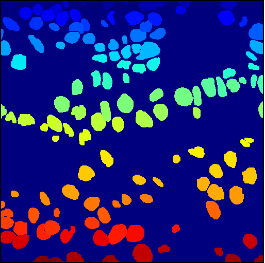
\includegraphics[width=4.0cm]{GT_1}}
%  \vspace{1.5cm}
  \centerline{Associated ground truth}\medskip
\end{minipage}
%
%
\begin{minipage}[b]{.48\linewidth}
  \centering
  \centerline{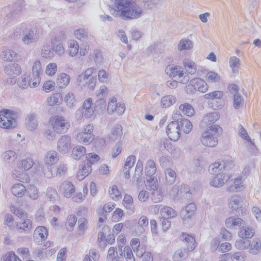
\includegraphics[width=4.0cm]{RGB_2}}
%  \vspace{1.5cm}
  \centerline{Sample from patient 581910}\medskip
\end{minipage}
\hfill
\begin{minipage}[b]{0.48\linewidth}
  \centering
  \centerline{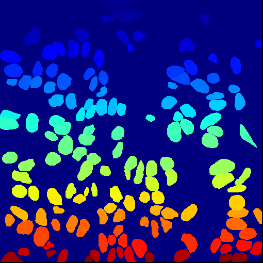
\includegraphics[width=4.0cm]{GT_2}}
%  \vspace{1.5cm}
  \centerline{Associated ground truth}\medskip
\end{minipage}
%
%
\begin{minipage}[b]{.48\linewidth}
  \centering
  \centerline{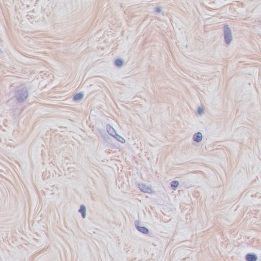
\includegraphics[width=4.0cm]{RGB_3}}
%  \vspace{1.5cm}
  \centerline{Another one from patient 581910}\medskip
\end{minipage}
\hfill
\begin{minipage}[b]{0.48\linewidth}
  \centering
  \centerline{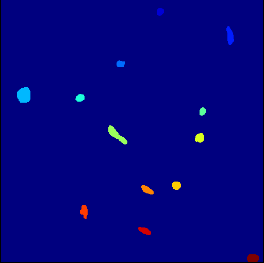
\includegraphics[width=4.0cm]{GT_3}}
%  \vspace{1.5cm}
  \centerline{Associated ground truth}\medskip
\end{minipage}
%
\caption{Random annotated samples from the dataset}
\label{fig:annotation}
%
\end{figure}


\begin{figure}[htb]
\begin{minipage}[b]{.48\linewidth}
  \centering
  \centerline{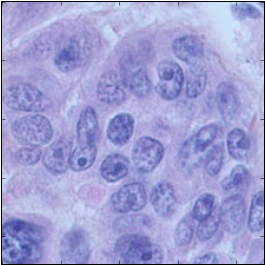
\includegraphics[height=4.0cm]{RGB_pred}}
%  \vspace{1.5cm}
  \centerline{Original RGB sample}\medskip
\end{minipage}
\hfill
\begin{minipage}[b]{0.48\linewidth}
  \centering
  \centerline{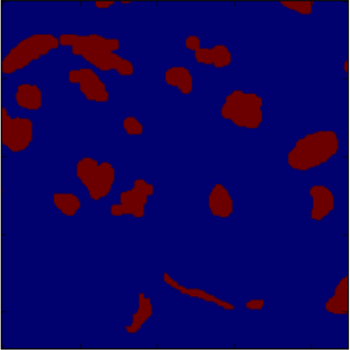
\includegraphics[width=4.0cm]{GT_pred}}
%  \vspace{1.5cm}
  \centerline{Associated ground truth}\medskip
\end{minipage}


\begin{minipage}[b]{0.48\linewidth}
  \centering
  \centerline{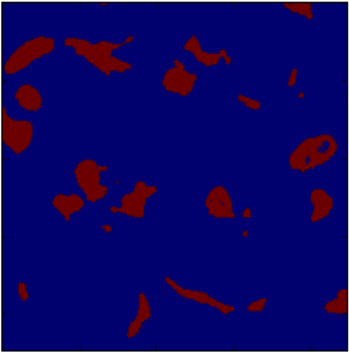
\includegraphics[height=4.0cm]{BaochuanB}}
%  \vspace{1.5cm}
  \centerline{PangNet}\medskip
\end{minipage}
\hfill
\begin{minipage}[b]{.48\linewidth}
  \centering
  \centerline{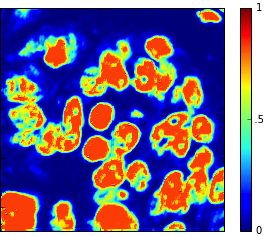
\includegraphics[height=4.0cm]{BaochuanP}}
%  \vspace{1.5cm}
  \centerline{Probability map}\medskip
\end{minipage}


%
%
\begin{minipage}[b]{.48\linewidth}
  \centering
  \centerline{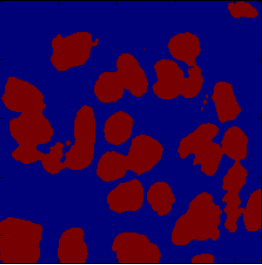
\includegraphics[height=4.0cm]{DeconvNetB}}
%  \vspace{1.5cm}
  \centerline{DeconvNet}\medskip
\end{minipage}
\hfill
\begin{minipage}[b]{0.48\linewidth}
  \centering
  \centerline{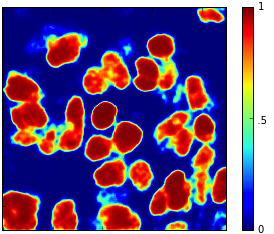
\includegraphics[height=4.0cm]{DeconvNetP}}
%  \vspace{1.5cm}
  \centerline{Probability map}\medskip
\end{minipage}
%
%
\begin{minipage}[b]{.48\linewidth}
  \centering
  \centerline{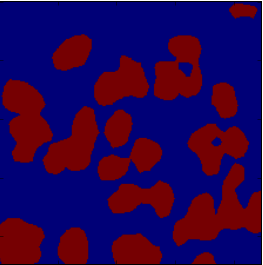
\includegraphics[height=4.0cm]{FCNB}}
%  \vspace{1.5cm}
  \centerline{FCN}\medskip
\end{minipage}
\hfill
\begin{minipage}[b]{0.48\linewidth}
  \centering
  \centerline{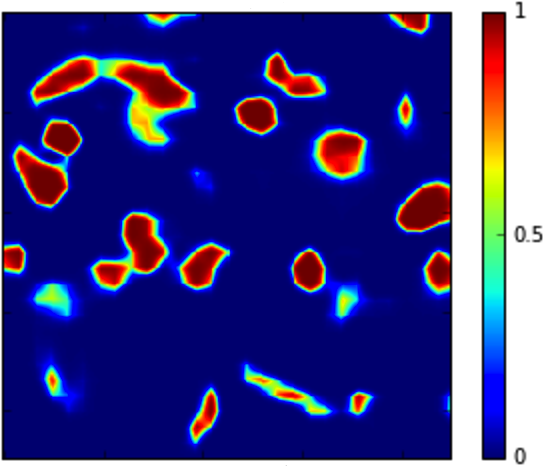
\includegraphics[height=4.0cm]{FCNP}}
%  \vspace{1.5cm}
  \centerline{Probability map}\medskip
\end{minipage}
%
\caption{Prediction via different classifiers of a random sample on the left out patient: 572123}
\label{fig:prediction}
%
\end{figure}

% To start a new column (but not a new page) and help balance the last-page
% column length use \vfill\pagebreak.
% -------------------------------------------------------------------------
\vfill
\pagebreak


%\section{FOOTNOTES}
%\label{sec:foot}
%
%Use footnotes sparingly (or not at all!) and place them at the bottom of the
%column on the page on which they are referenced. Use Times 9-point type,
%single-spaced. To help your readers, avoid using footnotes altogether and
%include necessary peripheral observations in the text (within parentheses, if
%you prefer, as in this sentence).
%

%\section{COPYRIGHT FORMS}
%\label{sec:copyright}
%
%You must include your fully completed, signed IEEE copyright release form when
%you submit your paper. We {\bf must} have this form before your paper can be
%published in the proceedings.  The copyright form is available as a Word file,
%a PDF file, and an HTML file. You can also use the form sent with your author
%kit.

%\section{REFERENCES}
%\label{sec:ref}

%List and number all bibliographical references at the end of the
%paper.  The references can be numbered in alphabetic order or in
%order of appearance in the document.  When referring to them in the
%text, type the corresponding reference number in square brackets as
%shown at the end of this sentence \cite{C2}. 

% References should be produced using the bibtex program from suitable
% BiBTeX files (here: strings, refs, manuals). The IEEEbib.bst bibliography
% style file from IEEE produces unsorted bibliography list.
% -------------------------------------------------------------------------
\bibliographystyle{IEEEbib}
\bibliography{refs}

\end{document}
